


\PassOptionsToPackage{xcolor}{usenames,dvipsnames,svgnames,table}
\documentclass[10pt]{report}
\usepackage[]{graphicx}\usepackage[]{xcolor}
%% maxwidth is the original width if it is less than linewidth
%% otherwise use linewidth (to make sure the graphics do not exceed the margin)
\makeatletter
\def\maxwidth{ %
  \ifdim\Gin@nat@width>\linewidth
    \linewidth
  \else
    \Gin@nat@width
  \fi
}
\makeatother

\definecolor{fgcolor}{rgb}{0.345, 0.345, 0.345}
\newcommand{\hlnum}[1]{\textcolor[rgb]{0.686,0.059,0.569}{#1}}%
\newcommand{\hlstr}[1]{\textcolor[rgb]{0.192,0.494,0.8}{#1}}%
\newcommand{\hlcom}[1]{\textcolor[rgb]{0.678,0.584,0.686}{\textit{#1}}}%
\newcommand{\hlopt}[1]{\textcolor[rgb]{0,0,0}{#1}}%
\newcommand{\hlstd}[1]{\textcolor[rgb]{0.345,0.345,0.345}{#1}}%
\newcommand{\hlkwa}[1]{\textcolor[rgb]{0.161,0.373,0.58}{\textbf{#1}}}%
\newcommand{\hlkwb}[1]{\textcolor[rgb]{0.69,0.353,0.396}{#1}}%
\newcommand{\hlkwc}[1]{\textcolor[rgb]{0.333,0.667,0.333}{#1}}%
\newcommand{\hlkwd}[1]{\textcolor[rgb]{0.737,0.353,0.396}{\textbf{#1}}}%

\usepackage{framed}
\makeatletter
\newenvironment{kframe}{%
 \def\at@end@of@kframe{}%
 \ifinner\ifhmode%
  \def\at@end@of@kframe{\end{minipage}}%
  \begin{minipage}{\columnwidth}%
 \fi\fi%
 \def\FrameCommand##1{\hskip\@totalleftmargin \hskip-\fboxsep
 \colorbox{shadecolor}{##1}\hskip-\fboxsep
     % There is no \\@totalrightmargin, so:
     \hskip-\linewidth \hskip-\@totalleftmargin \hskip\columnwidth}%
 \MakeFramed {\advance\hsize-\width
   \@totalleftmargin\z@ \linewidth\hsize
   \@setminipage}}%
 {\par\unskip\endMakeFramed%
 \at@end@of@kframe}
\makeatother

\definecolor{shadecolor}{rgb}{.97, .97, .97}
\definecolor{messagecolor}{rgb}{0, 0, 0}
\definecolor{warningcolor}{rgb}{1, 0, 1}
\definecolor{errorcolor}{rgb}{1, 0, 0}
\newenvironment{knitrout}{}{} % an empty environment to be redefined in TeX

\usepackage{alltt}
\newcommand{\SweaveOpts}[1]{}  % do not interfere with LaTeX
\newcommand{\SweaveInput}[1]{} % because they are not real TeX commands
\newcommand{\Sexpr}[1]{}       % will only be parsed by R


\usepackage[T1]{fontenc}
\usepackage{lmodern}
\usepackage{pdfcolmk}
\usepackage{multirow}
\usepackage{graphicx}
\usepackage{pifont}
\usepackage{amsmath,amsfonts,amsthm,amssymb}
\usepackage{setspace}
\usepackage{Tabbing}
\usepackage{etoolbox}
\usepackage{fancyhdr}
\usepackage{lastpage}
\usepackage{listings}
\usepackage{extramarks}
\usepackage{enumerate}
\usepackage{soul,color}
\usepackage{graphicx,float,wrapfig}
\usepackage{amsmath,amssymb,rotating}
\usepackage{epsfig}
\usepackage{color}
\usepackage{hyperref}
\usepackage{animate}
\usepackage{array}
\usepackage{graphics, color}
\usepackage{graphicx}
\usepackage{epsfig}
\usepackage{setspace}
\usepackage{verbatim}
\usepackage[margin=1.0in]{geometry}
\usepackage{tikz}
\usepackage{mdframed}
\usepackage{clrscode3e}
\usepackage{formalHW}
\usepackage[DMC,none]{formatHW}
\usepackage{fancyquote}
\usepackage{fancyenvironments}
\usepackage{mymathmacros}
\usepackage{algorithm}
\usepackage[noend]{algpseudocode}
\usepackage{pgfplots}





\begin{document}
% For LaTeX-Box: root = first_attempt.tex 
%%%%%%%%%%%%%%%%%%%%%%%%%%%%%%%%%%%%%%%%%%%%%%%%%%%%%%%%%%%%%%%%%%%%%%%%%%%%%%%%
%  File Name: first_attempt.rnw
%  Purpose:
%
%  Creation Date: 07-04-2015
%  Last Modified: Sun Apr 12 19:52:39 2015
%  Created By:
%%%%%%%%%%%%%%%%%%%%%%%%%%%%%%%%%%%%%%%%%%%%%%%%%%%%%%%%%%%%%%%%%%%%%%%%%%%%%%%%
%-- Set parent file


%-- title page and quote
\HWinfo{April 7 2015}{1}{}
\titleheader

I am using the following packages:
%-- paks: R code (Code in Document)
\begin{knitrout}
\definecolor{shadecolor}{rgb}{0.969, 0.969, 0.969}\color{fgcolor}\begin{kframe}
\begin{alltt}
\hlkwd{library}\hlstd{(ggplot2)}
\hlkwd{library}\hlstd{(lubridate)}
\hlkwd{library}\hlstd{(xtable)}
\hlkwd{library}\hlstd{(rCharts)}
\hlkwd{library}\hlstd{(plyr)}
\hlkwd{library}\hlstd{(reshape2)}
\end{alltt}
\end{kframe}
\end{knitrout}
and my working directory is set to \verb!dmc2015/ian!.

\section{Starting with the basics}
\subsection{Reading the data correctly}
The data is appears to be "pipe delimited", the same format used in the 2013 DMC. 
To be on the safe side we should possible scan the file first:
%-- scanData: R code (Code in Document)
\begin{knitrout}
\definecolor{shadecolor}{rgb}{0.969, 0.969, 0.969}\color{fgcolor}\begin{kframe}
\begin{alltt}
\hlcom{# scan the first five lines}
\hlstd{raw_file} \hlkwb{<-} \hlkwd{scan}\hlstd{(}\hlkwc{file} \hlstd{=} \hlstr{"../data/raw_data/DMC_2015_orders_class.txt"}\hlstd{,}
    \hlkwc{what} \hlstd{=} \hlstr{"character"}\hlstd{,} \hlkwc{nlines} \hlstd{=} \hlnum{5}\hlstd{,} \hlkwc{sep} \hlstd{=} \hlstr{"\textbackslash{}n"}\hlstd{,} \hlkwc{na.strings} \hlstd{=} \hlstr{""}\hlstd{)}
\hlstd{raw_file[}\hlnum{2}\hlstd{]}
\end{alltt}
\begin{verbatim}
## [1] "6054|2015-03-10 08:09:55|8877a81d04e853bc31c50da2bd2afaff|2015-03-10 08:03:09|a35974920ba3c9b3a6e50a89910e6b81|9.17|2.04|0.94|1|4e03e74099990e8529eb7e7328220af1|c06dc2b4a5f7ecdfa27a83acf7a29423|b7e3b0110f96213f5087034b92be487a,667daa357f8999be0805a6d62d7d3970|5d64a4abdded231d2b2bc310b13d4ed8|4.82|0.6|1.57|0||008b99d9c2fd9d58dd1483e364f8e8d3|f12c4112c9ea685dc2d2705b1448bfbc|1b950b8f844e60606af9a7afaad9e0d6|6.21|1.24|1.57|1|4e03e74099990e8529eb7e7328220af1|6cb9192a405cfe3283dc2dd4d1c8899b|796c5815752a170021838a78bf7fab34||||"
\end{verbatim}
\begin{alltt}
\hlstd{raw_file[}\hlnum{4}\hlstd{]}
\end{alltt}
\begin{verbatim}
## [1] "6056|2015-03-10 10:42:51|313124dadc91f974ef726b76f1c4d014|2015-03-10 09:51:31|bd25bbf47a12fdb71ca888450a770a57|7.83|1.73|0.94|0|f6601412b868a05c118961e9d7869bc8|920c97ba22e2235de589e5cc9b391709|b78123c345b9f8a300a7fac7a735a8bd,6f735673e0cbf770a14c38aa256011a7|9ba570a84b154eefaed3c491f7caf392|5.93|0.98|1.57|0|f6601412b868a05c118961e9d7869bc8|008b99d9c2fd9d58dd1483e364f8e8d3|f12c4112c9ea685dc2d2705b1448bfbc|daa1e02e3b7b8f55f30d5deb937ed906|3.33|2.38|0.63|1|4e03e74099990e8529eb7e7328220af1|719076d25a5d21b11a8534341545823b|796c5815752a170021838a78bf7fab34,667daa357f8999be0805a6d62d7d3970||||"
\end{verbatim}
\end{kframe}
\end{knitrout}
Notice that some of the variables have commas separating them. 
Additionally, there are \verb!||||! at the ends of the lines (the classification data is missing what we need to predict).

Read the data into R:
%-- readDat: R code (Code in Document)
\begin{knitrout}
\definecolor{shadecolor}{rgb}{0.969, 0.969, 0.969}\color{fgcolor}\begin{kframe}
\begin{alltt}
\hlcom{# training set ('historical data')}
\hlstd{trn} \hlkwb{<-} \hlkwd{read.delim}\hlstd{(}\hlstr{"../data/raw_data/DMC_2015_orders_train.txt"}\hlstd{,}
    \hlkwc{stringsAsFactors} \hlstd{=} \hlnum{FALSE}\hlstd{,} \hlkwc{sep} \hlstd{=} \hlstr{"|"}\hlstd{,} \hlkwc{quote} \hlstd{=} \hlstr{""}\hlstd{)}

\hlcom{# test set ('future data')}
\hlstd{tst} \hlkwb{<-} \hlkwd{read.delim}\hlstd{(}\hlstr{"../data/raw_data/DMC_2015_orders_class.txt"}\hlstd{,}
    \hlkwc{stringsAsFactors} \hlstd{=} \hlnum{FALSE}\hlstd{,} \hlkwc{sep} \hlstd{=} \hlstr{"|"}\hlstd{,} \hlkwc{quote} \hlstd{=} \hlstr{""}\hlstd{)}
\end{alltt}
\end{kframe}
\end{knitrout}

I will break up the data set into the following sets of columns for easy display:

\textbf{Session information}
The variables \verb!orderID!, \verb!orderTime!, \verb!userID!, and \verb!couponsReceived! are described as 
"order number", "time of order", "user identifier", and "time of coupon generation" respectively.
The response (?) \verb!basketValue! could also go here.
These variable all describe who was shopping and when.
%-- sessioninfo: R code (Code in Document)
\begin{kframe}
\begin{alltt}
\hlkwd{print}\hlstd{(}\hlkwd{xtable}\hlstd{(}\hlkwd{head}\hlstd{(trn[,} \hlkwd{c}\hlstd{(}\hlnum{1}\hlopt{:}\hlnum{4}\hlstd{,} \hlkwd{ncol}\hlstd{(trn))])),} \hlkwc{table.placement} \hlstd{=} \hlstr{"H"}\hlstd{)}
\end{alltt}
\end{kframe}% latex table generated in R 3.1.3 by xtable 1.7-4 package
% Sun Apr 12 19:52:43 2015
\begin{table}[H]
\centering
\begin{tabular}{rrlllr}
  \hline
 & orderID & orderTime & userID & couponsReceived & basketValue \\ 
  \hline
1 &   1 & 2015-01-06 09:38:35 & f77fdea046ce0a40eb30ac35dde882cd & 2015-01-06 09:34:53 & 187.60 \\ 
  2 &   2 & 2015-01-06 10:03:19 & 49fb109b47d0cee1753b63c24574d9d5 & 2015-01-06 10:00:44 & 185.93 \\ 
  3 &   3 & 2015-01-06 10:08:13 & b767e0e5cda30fc2e7c39f8049eebb5a & 2015-01-06 09:29:16 & 208.07 \\ 
  4 &   4 & 2015-01-06 13:23:23 & cae358d7b2d59aafe8e41e70b363a198 & 2015-01-06 13:13:12 & 185.80 \\ 
  5 &   5 & 2015-01-06 13:37:22 & 9ddbc3f477d31b609f962555d72503ad & 2015-01-06 12:48:41 & 272.12 \\ 
  6 &   6 & 2015-01-06 15:26:36 & 1c8dc3fa9ef6d8734fa26e5af8be0b0b & 2015-01-06 15:14:20 & 126.01 \\ 
   \hline
\end{tabular}
\end{table}


\textbf{Coupon 1, 2, and 3}
Each coupon has its own set of descriptors attached to it. For instance, coupon $i$ has 
\verb!couponIDi! (an ID), 
\verb!pricei! (the "current" price of the product to which coupon $i$ pertains),
\verb!basePricei! (the "original" price of the product to which coupon $i$ pertains),
\verb!rewardi! (the "score value" for the value-added of the product for the retailer)
\verb!premiumProducti! (indicates if the product is premium),
\verb!brandi! (the brand of the product),
\verb!productGroupi! (the "product line" of the product),
and
\verb!categoryIDsi! (identifies the categories of the first coupon product).
Finally, there is also \verb!couponiUsed!.
%-- sessioninfo: R code (Code in Document)

Coupon 1:
\begin{kframe}
\begin{alltt}
\hlkwd{print}\hlstd{(}\hlkwd{xtable}\hlstd{(}\hlkwd{head}\hlstd{(trn[,} \hlkwd{which}\hlstd{(}\hlkwd{grepl}\hlstd{(}\hlstr{"1"}\hlstd{,} \hlkwd{names}\hlstd{(trn)))[}\hlnum{1}\hlopt{:}\hlnum{5}\hlstd{]])),}
    \hlkwc{table.placement} \hlstd{=} \hlstr{"H"}\hlstd{)}
\end{alltt}
\end{kframe}% latex table generated in R 3.1.3 by xtable 1.7-4 package
% Sun Apr 12 19:52:43 2015
\begin{table}[H]
\centering
\begin{tabular}{rlrrrr}
  \hline
 & couponID1 & price1 & basePrice1 & reward1 & premiumProduct1 \\ 
  \hline
1 & 89d62b666d585f03f262b1f6a6abdd2c & 3.24 & 5.40 & 1.57 &   0 \\ 
  2 & 093c94d44333cd07a4318a0231b967c8 & 2.32 & 1.59 & 1.57 &   0 \\ 
  3 & a10bb278883972b3e977d30f4c5d526c & 7.92 & 2.64 & 1.26 &   1 \\ 
  4 & 0a0a18c1985e5a2580968bbc90492574 & 2.50 & 2.08 & 1.57 &   0 \\ 
  5 & f6e2fa236e98883e972bf0fc58f292e6 & 12.27 & 2.45 & 1.26 &   0 \\ 
  6 & a6f321b6e5cdc83deb463f46d1921df2 & 7.50 & 1.25 & 0.63 &   0 \\ 
   \hline
\end{tabular}
\end{table}
\begin{kframe}\begin{alltt}
\hlkwd{print}\hlstd{(}\hlkwd{xtable}\hlstd{(}\hlkwd{head}\hlstd{(trn[,} \hlkwd{which}\hlstd{(}\hlkwd{grepl}\hlstd{(}\hlstr{"1"}\hlstd{,} \hlkwd{names}\hlstd{(trn)))[}\hlnum{6}\hlopt{:}\hlnum{7}\hlstd{]])),}
    \hlkwc{table.placement} \hlstd{=} \hlstr{"H"}\hlstd{)}
\end{alltt}
\end{kframe}% latex table generated in R 3.1.3 by xtable 1.7-4 package
% Sun Apr 12 19:52:43 2015
\begin{table}[H]
\centering
\begin{tabular}{rll}
  \hline
 & brand1 & productGroup1 \\ 
  \hline
1 & 788c2fd7ba973489e6529275c01211db & bfdca7185ad7366f965590bab1417db5 \\ 
  2 & f6601412b868a05c118961e9d7869bc8 & e8f2ae4556952195821c46ea2da1d21c \\ 
  3 & 4e03e74099990e8529eb7e7328220af1 & c06dc2b4a5f7ecdfa27a83acf7a29423 \\ 
  4 & a38b030516e52b6f126fb96c159aba25 & ff897252b17f195b5216eef189a775ab \\ 
  5 & a38b030516e52b6f126fb96c159aba25 & c06dc2b4a5f7ecdfa27a83acf7a29423 \\ 
  6 & f6601412b868a05c118961e9d7869bc8 & 113593efe095675415192b4aa1ab8653 \\ 
   \hline
\end{tabular}
\end{table}
\begin{kframe}\begin{alltt}
\hlkwd{print}\hlstd{(}\hlkwd{xtable}\hlstd{(}\hlkwd{head}\hlstd{(trn[,} \hlkwd{which}\hlstd{(}\hlkwd{grepl}\hlstd{(}\hlstr{"1"}\hlstd{,} \hlkwd{names}\hlstd{(trn)))[}\hlnum{8}\hlopt{:}\hlnum{9}\hlstd{]])),}
    \hlkwc{table.placement} \hlstd{=} \hlstr{"H"}\hlstd{)}
\end{alltt}
\end{kframe}% latex table generated in R 3.1.3 by xtable 1.7-4 package
% Sun Apr 12 19:52:43 2015
\begin{table}[H]
\centering
\begin{tabular}{rlr}
  \hline
 & categoryIDs1 & coupon1Used \\ 
  \hline
1 & b7e3b0110f96213f5087034b92be487a,4b3e2dbd4d59c43bf6982405a5f7fce7 &   0 \\ 
  2 & 796c5815752a170021838a78bf7fab34 &   1 \\ 
  3 & b7e3b0110f96213f5087034b92be487a,667daa357f8999be0805a6d62d7d3970 &   0 \\ 
  4 & b7e3b0110f96213f5087034b92be487a &   1 \\ 
  5 & b7e3b0110f96213f5087034b92be487a &   0 \\ 
  6 & b78123c345b9f8a300a7fac7a735a8bd,6f735673e0cbf770a14c38aa256011a7 &   1 \\ 
   \hline
\end{tabular}
\end{table}


Coupon 2:
\begin{kframe}
\begin{alltt}
\hlkwd{print}\hlstd{(}\hlkwd{xtable}\hlstd{(}\hlkwd{head}\hlstd{(trn[,} \hlkwd{which}\hlstd{(}\hlkwd{grepl}\hlstd{(}\hlstr{"2"}\hlstd{,} \hlkwd{names}\hlstd{(trn)))[}\hlnum{1}\hlopt{:}\hlnum{5}\hlstd{]])),}
    \hlkwc{table.placement} \hlstd{=} \hlstr{"H"}\hlstd{)}
\end{alltt}
\end{kframe}% latex table generated in R 3.1.3 by xtable 1.7-4 package
% Sun Apr 12 19:52:43 2015
\begin{table}[H]
\centering
\begin{tabular}{rlrrrr}
  \hline
 & couponID2 & price2 & basePrice2 & reward2 & premiumProduct2 \\ 
  \hline
1 & f2d9a4e781b3f198f244d6c130152bb8 & 5.19 & 0.57 & 1.57 &   0 \\ 
  2 & 4947578494e36ec93b27470bf0d9b868 & 3.70 & 1.85 & 0.94 &   0 \\ 
  3 & af9837e0d8f484f3520285f3d5f3deb7 & 4.17 & 1.39 & 1.26 &   1 \\ 
  4 & edba887265f47c8dde81e0a24d472519 & 3.66 & 0.73 & 1.57 &   1 \\ 
  5 & 179e167fd0dc215ddf6346999a1d8ba6 & 5.74 & 0.88 & 1.57 &   1 \\ 
  6 & 7d6c167459169a4ad31357870b1f70fe & 4.35 & 1.44 & 1.26 &   0 \\ 
   \hline
\end{tabular}
\end{table}
\begin{kframe}\begin{alltt}
\hlkwd{print}\hlstd{(}\hlkwd{xtable}\hlstd{(}\hlkwd{head}\hlstd{(trn[,} \hlkwd{which}\hlstd{(}\hlkwd{grepl}\hlstd{(}\hlstr{"2"}\hlstd{,} \hlkwd{names}\hlstd{(trn)))[}\hlnum{6}\hlopt{:}\hlnum{7}\hlstd{]])),}
    \hlkwc{table.placement} \hlstd{=} \hlstr{"H"}\hlstd{)}
\end{alltt}
\end{kframe}% latex table generated in R 3.1.3 by xtable 1.7-4 package
% Sun Apr 12 19:52:43 2015
\begin{table}[H]
\centering
\begin{tabular}{rll}
  \hline
 & brand2 & productGroup2 \\ 
  \hline
1 & f6601412b868a05c118961e9d7869bc8 & 041a02d031057ba1c2e210fe6b0db0f4 \\ 
  2 &  & fa5cc31a659b346bcb8c069991fcd326 \\ 
  3 & 4e03e74099990e8529eb7e7328220af1 & 7ebc31798e2d38e862cc336f448781a9 \\ 
  4 & 4e03e74099990e8529eb7e7328220af1 & 008b99d9c2fd9d58dd1483e364f8e8d3 \\ 
  5 & 4e03e74099990e8529eb7e7328220af1 & e54573aaf3c08c40545b97cc5ddf1732 \\ 
  6 &  & fee2c21073bf07c9cd87566fe98fcfb2 \\ 
   \hline
\end{tabular}
\end{table}
\begin{kframe}\begin{alltt}
\hlkwd{print}\hlstd{(}\hlkwd{xtable}\hlstd{(}\hlkwd{head}\hlstd{(trn[,} \hlkwd{which}\hlstd{(}\hlkwd{grepl}\hlstd{(}\hlstr{"2"}\hlstd{,} \hlkwd{names}\hlstd{(trn)))[}\hlnum{8}\hlopt{:}\hlnum{9}\hlstd{]])),}
    \hlkwc{table.placement} \hlstd{=} \hlstr{"H"}\hlstd{)}
\end{alltt}
\end{kframe}% latex table generated in R 3.1.3 by xtable 1.7-4 package
% Sun Apr 12 19:52:43 2015
\begin{table}[H]
\centering
\begin{tabular}{rlr}
  \hline
 & categoryIDs2 & coupon2Used \\ 
  \hline
1 & f12c4112c9ea685dc2d2705b1448bfbc,a0ae3bad823bea2ffa642bf47daa4a77 &   1 \\ 
  2 & f929d7624d13f00e1ca52c9edb5c03ba &   0 \\ 
  3 & f12c4112c9ea685dc2d2705b1448bfbc,667daa357f8999be0805a6d62d7d3970 &   0 \\ 
  4 & f12c4112c9ea685dc2d2705b1448bfbc,667daa357f8999be0805a6d62d7d3970,a0ae3bad823bea2ffa642bf47daa4a77 &   1 \\ 
  5 & f12c4112c9ea685dc2d2705b1448bfbc,667daa357f8999be0805a6d62d7d3970 &   0 \\ 
  6 & 7a04f5ee0a1363e6af5ca20434ed72a0,4b3e2dbd4d59c43bf6982405a5f7fce7 &   0 \\ 
   \hline
\end{tabular}
\end{table}


Coupon 3:
\begin{kframe}
\begin{alltt}
\hlkwd{print}\hlstd{(}\hlkwd{xtable}\hlstd{(}\hlkwd{head}\hlstd{(trn[,} \hlkwd{which}\hlstd{(}\hlkwd{grepl}\hlstd{(}\hlstr{"3"}\hlstd{,} \hlkwd{names}\hlstd{(trn)))[}\hlnum{1}\hlopt{:}\hlnum{5}\hlstd{]])),}
    \hlkwc{table.placement} \hlstd{=} \hlstr{"H"}\hlstd{)}
\end{alltt}
\end{kframe}% latex table generated in R 3.1.3 by xtable 1.7-4 package
% Sun Apr 12 19:52:43 2015
\begin{table}[H]
\centering
\begin{tabular}{rlrrrr}
  \hline
 & couponID3 & price3 & basePrice3 & reward3 & premiumProduct3 \\ 
  \hline
1 & bd6402915feb3dd717c579f3f133ba22 & 12.92 & 12.92 & 2.20 &   0 \\ 
  2 & 7d105576cee40e8f9ffd798903c9da81 & 3.89 & 0.06 & 2.20 &   0 \\ 
  3 & 4270374b0780f856a6afdf98bf759f1a & 2.73 & 0.88 & 1.26 &   0 \\ 
  4 & 5de73019819ae0aafb3d8224b0686558 & 5.74 & 4.25 & 1.57 &   0 \\ 
  5 & 4430e468db7670b2ffbefd6cdb9d89e3 & 4.91 & 2.45 & 1.57 &   1 \\ 
  6 & 476adba5b863c0bde731b9fb9b18e64b & 5.51 & 1.43 & 3.14 &   0 \\ 
   \hline
\end{tabular}
\end{table}
\begin{kframe}\begin{alltt}
\hlkwd{print}\hlstd{(}\hlkwd{xtable}\hlstd{(}\hlkwd{head}\hlstd{(trn[,} \hlkwd{which}\hlstd{(}\hlkwd{grepl}\hlstd{(}\hlstr{"3"}\hlstd{,} \hlkwd{names}\hlstd{(trn)))[}\hlnum{6}\hlopt{:}\hlnum{7}\hlstd{]])),}
    \hlkwc{table.placement} \hlstd{=} \hlstr{"H"}\hlstd{)}
\end{alltt}
\end{kframe}% latex table generated in R 3.1.3 by xtable 1.7-4 package
% Sun Apr 12 19:52:43 2015
\begin{table}[H]
\centering
\begin{tabular}{rll}
  \hline
 & brand3 & productGroup3 \\ 
  \hline
1 &  & 94a7d11a8972ed94819c748a1d1b42f8 \\ 
  2 & f6601412b868a05c118961e9d7869bc8 & f5d6f7cd5f84fd41fbc4535f0fb77b89 \\ 
  3 & 304979e999d95fc59d85cba5f1633595 & e006513b5c7be290e81c8bd614362d07 \\ 
  4 & 304979e999d95fc59d85cba5f1633595 & b1f57b4c3876f032a2b0ea1f714b0940 \\ 
  5 & 4e03e74099990e8529eb7e7328220af1 & d1b083d764bac332ee2715c369cf7ec1 \\ 
  6 &  & 5d7f92459adc7208db382fdf5d8f5896 \\ 
   \hline
\end{tabular}
\end{table}
\begin{kframe}\begin{alltt}
\hlkwd{print}\hlstd{(}\hlkwd{xtable}\hlstd{(}\hlkwd{head}\hlstd{(trn[,} \hlkwd{which}\hlstd{(}\hlkwd{grepl}\hlstd{(}\hlstr{"3"}\hlstd{,} \hlkwd{names}\hlstd{(trn)))[}\hlnum{8}\hlopt{:}\hlnum{9}\hlstd{]])),}
    \hlkwc{table.placement} \hlstd{=} \hlstr{"H"}\hlstd{)}
\end{alltt}
\end{kframe}% latex table generated in R 3.1.3 by xtable 1.7-4 package
% Sun Apr 12 19:52:43 2015
\begin{table}[H]
\centering
\begin{tabular}{rlr}
  \hline
 & categoryIDs3 & coupon3Used \\ 
  \hline
1 & 796c5815752a170021838a78bf7fab34,a0ae3bad823bea2ffa642bf47daa4a77,4b3e2dbd4d59c43bf6982405a5f7fce7 &   0 \\ 
  2 & f929d7624d13f00e1ca52c9edb5c03ba &   1 \\ 
  3 & 796c5815752a170021838a78bf7fab34,4b3e2dbd4d59c43bf6982405a5f7fce7 &   0 \\ 
  4 & 796c5815752a170021838a78bf7fab34,4b3e2dbd4d59c43bf6982405a5f7fce7 &   0 \\ 
  5 & 796c5815752a170021838a78bf7fab34 &   0 \\ 
  6 & 796c5815752a170021838a78bf7fab34 &   1 \\ 
   \hline
\end{tabular}
\end{table}



\section{Exploring the Data}
\subsection{Session information}
 
There are two time variables which could be better formatted using \verb!lubridate!.
Additionally, it allows us to extract the time, date, and the day of the week separately.
I add an indicator for weekend instead of weekday and Friday/Saturday vs the rest of the week.
I wrote this function so that it could be done quickly for both variables in the training
and in the test set:
%-- manageTime: R code (Code in Document)
\begin{knitrout}
\definecolor{shadecolor}{rgb}{0.969, 0.969, 0.969}\color{fgcolor}\begin{kframe}
\begin{alltt}
\hlstd{TimeFeatures} \hlkwb{<-} \hlkwa{function}\hlstd{(}\hlkwc{dsn}\hlstd{,} \hlkwc{varn}\hlstd{) \{}
    \hlcom{# don't overwrite you data}
    \hlkwd{stopifnot}\hlstd{(}\hlopt{!}\hlstd{(}\hlkwd{paste0}\hlstd{(varn,} \hlstr{"DoW"}\hlstd{)} \hlopt \hlkwd{names}\hlstd{(dsn)))}

    \hlcom{# store time variables in this set}
    \hlstd{dsn.time} \hlkwb{<-} \hlstd{dsn[,} \hlkwd{c}\hlstd{(}\hlstr{"orderID"}\hlstd{, varn)]}

    \hlcom{# add information about order dates}
    \hlstd{dsn.time[, varn]} \hlkwb{<-} \hlkwd{ymd_hms}\hlstd{(dsn.time[, varn],} \hlkwc{tz} \hlstd{=} \hlstr{"CET"}\hlstd{)}

    \hlcom{# split the date-time variable into date and time}
    \hlstd{timedate} \hlkwb{<-} \hlkwd{ldply}\hlstd{(}\hlkwd{strsplit}\hlstd{(dsn[, varn],} \hlstr{" "}\hlstd{))}

    \hlcom{# get time of day, date, and day of week alone}
    \hlstd{dsn.time}\hlopt{$}\hlstd{Date} \hlkwb{<-} \hlkwd{ymd}\hlstd{(timedate[,} \hlnum{1}\hlstd{])}
    \hlstd{dsn.time}\hlopt{$}\hlstd{Time} \hlkwb{<-} \hlkwd{hms}\hlstd{(timedate[,} \hlnum{2}\hlstd{])}

    \hlcom{# get the day of the week}
    \hlstd{dsn.time}\hlopt{$}\hlstd{DoW} \hlkwb{<-} \hlkwd{wday}\hlstd{(dsn.time[, varn],} \hlkwc{label} \hlstd{=} \hlnum{TRUE}\hlstd{,}
        \hlkwc{abbr} \hlstd{=} \hlnum{FALSE}\hlstd{)}

    \hlcom{# weekend or preweekend indicators}
    \hlstd{dsn.time}\hlopt{$}\hlstd{Weekend} \hlkwb{<-} \hlkwd{factor}\hlstd{(}\hlnum{1} \hlopt{*} \hlstd{(dsn.time}\hlopt{$}\hlstd{DoW} \hlopt
        \hlkwd{c}\hlstd{(}\hlstr{"Saturday"}\hlstd{,} \hlstr{"Sunday"}\hlstd{)))}
    \hlstd{dsn.time}\hlopt{$}\hlstd{FriSat} \hlkwb{<-} \hlkwd{factor}\hlstd{(}\hlnum{1} \hlopt{*} \hlstd{(dsn.time}\hlopt{$}\hlstd{DoW} \hlopt
        \hlkwd{c}\hlstd{(}\hlstr{"Friday"}\hlstd{,} \hlstr{"Saturday"}\hlstd{)))}

    \hlcom{# merge with original data set}
    \hlkwd{names}\hlstd{(dsn.time)[}\hlopt{-}\hlkwd{c}\hlstd{(}\hlnum{1}\hlopt{:}\hlnum{2}\hlstd{)]} \hlkwb{<-} \hlkwd{paste0}\hlstd{(varn,} \hlkwd{names}\hlstd{(dsn.time)[}\hlopt{-}\hlkwd{c}\hlstd{(}\hlnum{1}\hlopt{:}\hlnum{2}\hlstd{)])}

    \hlstd{dsn} \hlkwb{<-} \hlkwd{merge}\hlstd{(dsn.time, dsn[,} \hlkwd{names}\hlstd{(dsn)} \hlopt{!=} \hlstd{varn],}
        \hlkwc{by} \hlstd{=} \hlstr{"orderID"}\hlstd{)}
    \hlkwd{return}\hlstd{(dsn)}
\hlstd{\}}

\hlcom{# Whatever you do to the training set}
\hlstd{trn} \hlkwb{<-} \hlkwd{TimeFeatures}\hlstd{(trn,} \hlstr{"orderTime"}\hlstd{)}
\hlstd{trn} \hlkwb{<-} \hlkwd{TimeFeatures}\hlstd{(trn,} \hlstr{"couponsReceived"}\hlstd{)}

\hlcom{# try if you can to do the same to the test set}
\hlstd{tst} \hlkwb{<-} \hlkwd{TimeFeatures}\hlstd{(tst,} \hlstr{"orderTime"}\hlstd{)}
\hlstd{tst} \hlkwb{<-} \hlkwd{TimeFeatures}\hlstd{(tst,} \hlstr{"couponsReceived"}\hlstd{)}
\end{alltt}
\end{kframe}
\end{knitrout}

Now that we have created the time variable as a backbone, 
we can make some interesting plots:
%-- R figure (code in document - set include=FALSE to remove)

Also notice that orders are numbered as they made.
\begin{knitrout}
\definecolor{shadecolor}{rgb}{0.969, 0.969, 0.969}\color{fgcolor}\begin{kframe}
\begin{alltt}
\hlkwd{qplot}\hlstd{(orderTime, orderID,} \hlkwc{data} \hlstd{= trn)}
\end{alltt}
\end{kframe}\begin{figure}[H]

{\centering 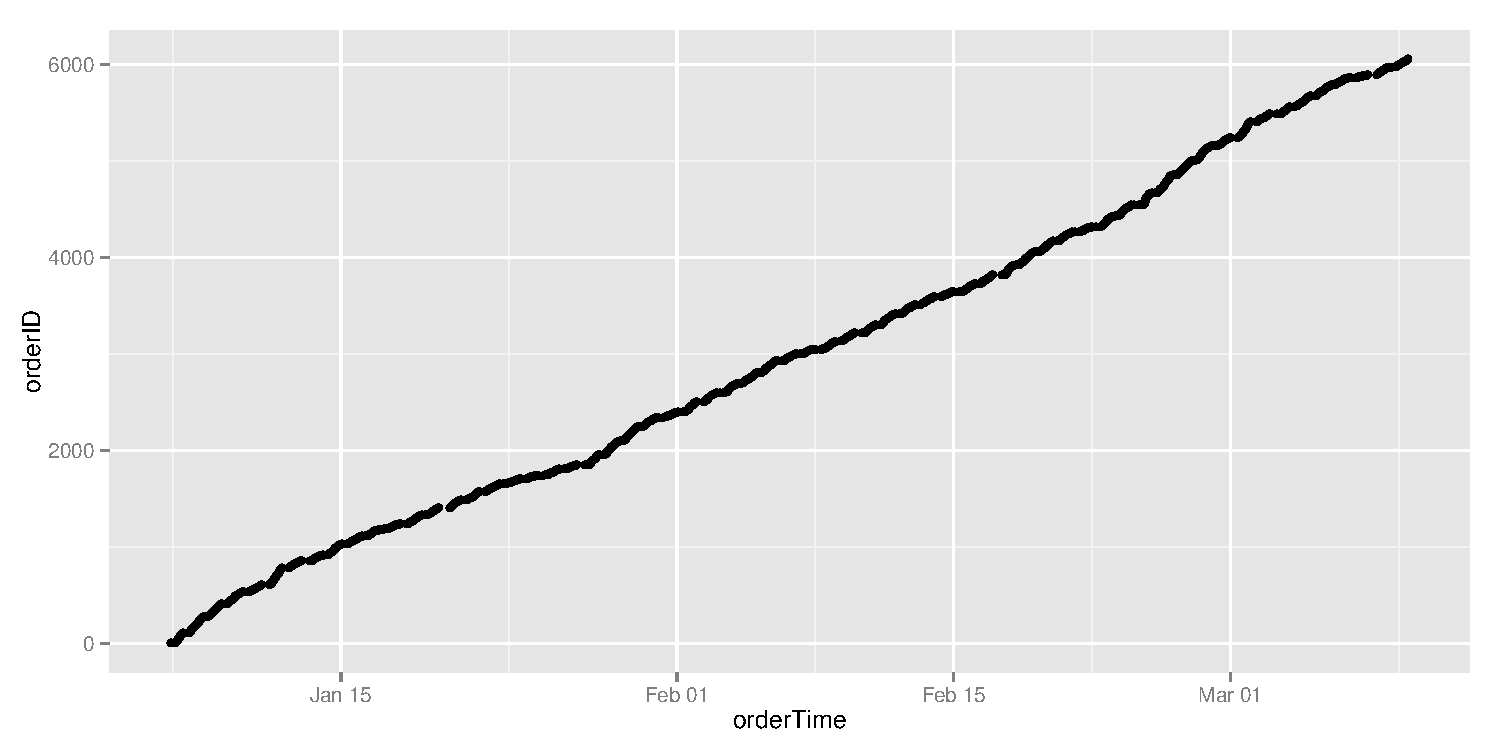
\includegraphics[width=.9\linewidth]{/Users/user/dmc2015/ian/graphics/graphics_unnamed-chunk-1-1} 

}

\caption[As time passes, new orders are processed]{As time passes, new orders are processed.  Notice that the number of new orders is generally smooth, indicating that customers are buying items consistently.}\label{fig:unnamed-chunk-1}
\end{figure}


\end{knitrout}
We can verify that orders are numbered in increasing order through time:
%-- R code (Code in Document)
\begin{knitrout}
\definecolor{shadecolor}{rgb}{0.969, 0.969, 0.969}\color{fgcolor}\begin{kframe}
\begin{alltt}
\hlkwd{sum}\hlstd{(}\hlkwd{sapply}\hlstd{(}\hlnum{1}\hlopt{:}\hlkwd{nrow}\hlstd{(trn),} \hlkwa{function}\hlstd{(}\hlkwc{i}\hlstd{)} \hlkwd{sum}\hlstd{(trn}\hlopt{$}\hlstd{orderTime[i]} \hlopt{<}
    \hlstd{trn}\hlopt{$}\hlstd{orderTime} \hlopt{&} \hlstd{trn}\hlopt{$}\hlstd{orderID[i]} \hlopt{>} \hlstd{trn}\hlopt{$}\hlstd{orderID)))}
\end{alltt}
\begin{verbatim}
## [1] 0
\end{verbatim}
\end{kframe}
\end{knitrout}

This creates a bit of a puzzle in our next plot:

\begin{knitrout}
\definecolor{shadecolor}{rgb}{0.969, 0.969, 0.969}\color{fgcolor}\begin{kframe}
\begin{alltt}
\hlkwd{qplot}\hlstd{(couponsReceived, orderTime,} \hlkwc{data} \hlstd{= trn)}
\end{alltt}
\end{kframe}\begin{figure}[H]

{\centering 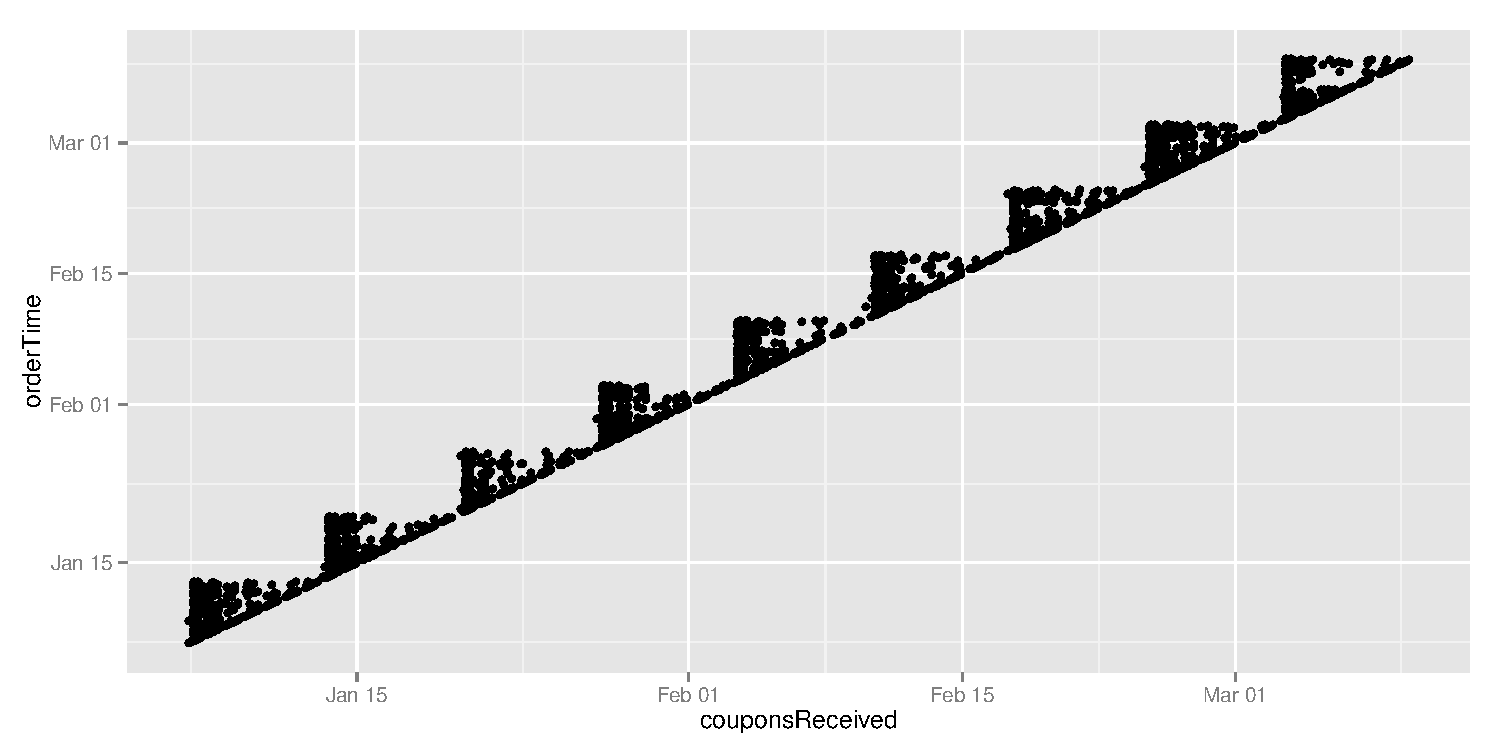
\includegraphics[width=.9\linewidth]{/Users/user/dmc2015/ian/graphics/graphics_unnamed-chunk-3-1} 

}

\caption[Orders alway follow receiving of coupons, but the odd shapes indicate that there is structure to the data beyond the fact that shoppers get coupons before purchasing any products]{Orders alway follow receiving of coupons, but the odd shapes indicate that there is structure to the data beyond the fact that shoppers get coupons before purchasing any products.}\label{fig:unnamed-chunk-3}
\end{figure}


\end{knitrout}

It seems that customers can not use coupons indefinetly. 
In fact, the difference between two points never exceeds  one week.
%-- nnss: R code (Code in Document)
\begin{knitrout}
\definecolor{shadecolor}{rgb}{0.969, 0.969, 0.969}\color{fgcolor}\begin{kframe}
\begin{alltt}
\hlcom{# longest time to act on coupon}
\hlkwd{max}\hlstd{(}\hlkwd{difftime}\hlstd{(trn}\hlopt{$}\hlstd{orderTime, trn}\hlopt{$}\hlstd{couponsReceived,} \hlkwc{units} \hlstd{=} \hlstr{"days"}\hlstd{))}
\end{alltt}
\begin{verbatim}
## Time difference of 6.401204 days
\end{verbatim}
\begin{alltt}
\hlcom{# shortest time to act on coupon}
\hlkwd{min}\hlstd{(}\hlkwd{difftime}\hlstd{(trn}\hlopt{$}\hlstd{orderTime, trn}\hlopt{$}\hlstd{couponsReceived,} \hlkwc{units} \hlstd{=} \hlstr{"secs"}\hlstd{))}
\end{alltt}
\begin{verbatim}
## Time difference of 6 secs
\end{verbatim}
\end{kframe}
\end{knitrout}
The earliest a fastest a customer acts on a coupon is 6 seconds!
Lets consider the possibility that customers are receiving coupons in gigantic batches.
Then it makes sense that the coupons will have one-week limits, and then a new batch of coupons are sent out.
For example, if we take the first time and add 7 days, any customer receiving coupons has only until
the 7th day after any customer in that batch receives a coupon to place an order.

We can use this idea to demarcate time into batches. 
This function assumes 
\begin{itemize}
   \item Coupons are sent in batches
\item Coupons are sent at the same time
\item A person has 7 days after the coupons are sent to use them, regardless of when the coupon is "received"
\end{itemize}

In addition to batchID, we can add the "pseudo-expiration" date of the coupon and "date sent" variables to our data:
%-- batches: R code (Code in Document) 
\begin{knitrout}
\definecolor{shadecolor}{rgb}{0.969, 0.969, 0.969}\color{fgcolor}\begin{kframe}
\begin{alltt}
\hlstd{GetBatchInfo} \hlkwb{<-} \hlkwa{function}\hlstd{(}\hlkwc{initial_batch.ymd_hms}\hlstd{,} \hlkwc{nbatch} \hlstd{=} \hlnum{10}\hlstd{,}
    \hlkwc{weeks2expire} \hlstd{=} \hlnum{1}\hlstd{,} \hlkwc{train} \hlstd{= trn,} \hlkwc{test} \hlstd{= tst) \{}
    \hlcom{# start sending coupons: initial_batch.ymd_hms =}
    \hlcom{# '2015-01-06 1:00:00' initial_batch.ymd_hms =}
    \hlcom{# '2015-01-03 1:00:00' How many batches are there?}
    \hlcom{# nbatch = 10 how long are coupons valid?}
    \hlcom{# weeks2expire = 1 what is the training set?  train}
    \hlcom{# = trn what is the test set?  test = tst}

    \hlkwd{require}\hlstd{(lubridate)}
    \hlkwd{stopifnot}\hlstd{(}\hlkwd{is.POSIXct}\hlstd{(}\hlkwd{ymd_hms}\hlstd{(initial_batch.ymd_hms))} \hlopt{&}
        \hlkwd{is.POSIXt}\hlstd{(}\hlkwd{ymd_hms}\hlstd{(initial_batch.ymd_hms)))}

    \hlcom{# expiration date one week after coupons are sent}
    \hlstd{couponLengthValid} \hlkwb{<-} \hlkwd{weeks}\hlstd{(weeks2expire)}

    \hlcom{# batches go out when the last batch expires}
    \hlstd{weeksbtwnbatches} \hlkwb{<-} \hlstd{weeks2expire}

    \hlcom{# coupons start on}
    \hlstd{batch.start} \hlkwb{<-} \hlkwd{ymd_hms}\hlstd{(initial_batch.ymd_hms,} \hlkwc{tz} \hlstd{=} \hlstr{"CET"}\hlstd{)}

    \hlcom{# make data frame}
    \hlstd{couponBatches} \hlkwb{<-} \hlkwd{data.frame}\hlstd{(}\hlkwc{sendDate} \hlstd{= batch.start} \hlopt{+}
        \hlstd{(}\hlnum{0}\hlopt{:}\hlstd{(nbatch} \hlopt{-} \hlnum{1}\hlstd{))} \hlopt{*} \hlstd{couponLengthValid,} \hlkwc{expireDate} \hlstd{= batch.start} \hlopt{+}
        \hlnum{1}\hlopt{:}\hlstd{nbatch} \hlopt{*} \hlstd{couponLengthValid,} \hlkwc{batch} \hlstd{=} \hlkwd{factor}\hlstd{(}\hlnum{1}\hlopt{:}\hlstd{nbatch))}

    \hlcom{# create time interval}
    \hlstd{couponBatches}\hlopt{$}\hlstd{validInterval} \hlkwb{<-} \hlkwd{with}\hlstd{(couponBatches,}
        \hlkwd{interval}\hlstd{(sendDate, expireDate))}

    \hlcom{# give the training set batchID}
    \hlstd{train}\hlopt{$}\hlstd{batchID} \hlkwb{<-} \hlnum{0}
    \hlstd{train}\hlopt{$}\hlstd{couponsExpire} \hlkwb{<-} \hlstd{batch.start} \hlopt{+} \hlkwd{years}\hlstd{(}\hlnum{1}\hlstd{)}
    \hlstd{train}\hlopt{$}\hlstd{couponsSent} \hlkwb{<-} \hlstd{batch.start}
    \hlkwa{for} \hlstd{(i} \hlkwa{in} \hlnum{1}\hlopt{:}\hlstd{nbatch) \{}
        \hlstd{orderinbatch} \hlkwb{<-} \hlstd{train}\hlopt{$}\hlstd{orderTime} \hlopt \hlstd{couponBatches}\hlopt{$}\hlstd{validInterval[i]} \hlopt{&}
            \hlstd{train}\hlopt{$}\hlstd{couponsReceived} \hlopt \hlstd{couponBatches}\hlopt{$}\hlstd{validInterval[i]}
        \hlstd{couponinbatch} \hlkwb{<-} \hlstd{train}\hlopt{$}\hlstd{couponsReceived} \hlopt
            \hlstd{couponBatches}\hlopt{$}\hlstd{validInterval[i]}
        \hlkwa{if} \hlstd{(}\hlkwd{sum}\hlstd{(orderinbatch)} \hlopt{>} \hlnum{0}\hlstd{)}
            \hlstd{train}\hlopt{$}\hlstd{batchID[orderinbatch]} \hlkwb{<-} \hlstd{couponBatches}\hlopt{$}\hlstd{batch[i]}
        \hlkwa{if} \hlstd{(}\hlkwd{sum}\hlstd{(couponinbatch)} \hlopt{>} \hlnum{0}\hlstd{) \{}
            \hlstd{train}\hlopt{$}\hlstd{couponsSent[couponinbatch]} \hlkwb{<-} \hlstd{couponBatches}\hlopt{$}\hlstd{couponsSent[i]}
            \hlstd{train}\hlopt{$}\hlstd{couponsExpire[couponinbatch]} \hlkwb{<-} \hlstd{couponBatches}\hlopt{$}\hlstd{couponsExpire[i]}
        \hlstd{\}}
    \hlstd{\}}
    \hlstd{train}\hlopt{$}\hlstd{batchID} \hlkwb{<-} \hlkwd{as.factor}\hlstd{(train}\hlopt{$}\hlstd{batchID)}
    \hlstd{train}\hlopt{$}\hlstd{dataset} \hlkwb{<-} \hlstr{"train"}

    \hlstd{test}\hlopt{$}\hlstd{batchID} \hlkwb{<-} \hlnum{0}
    \hlstd{test}\hlopt{$}\hlstd{couponsExpire} \hlkwb{<-} \hlstd{batch.start} \hlopt{+} \hlkwd{years}\hlstd{(}\hlnum{1}\hlstd{)}
    \hlstd{test}\hlopt{$}\hlstd{couponsSent} \hlkwb{<-} \hlstd{batch.start}
    \hlkwa{for} \hlstd{(i} \hlkwa{in} \hlnum{1}\hlopt{:}\hlstd{nbatch) \{}
        \hlstd{orderinbatch} \hlkwb{<-} \hlstd{test}\hlopt{$}\hlstd{orderTime} \hlopt \hlstd{couponBatches}\hlopt{$}\hlstd{validInterval[i]} \hlopt{&}
            \hlstd{test}\hlopt{$}\hlstd{couponsReceived} \hlopt \hlstd{couponBatches}\hlopt{$}\hlstd{validInterval[i]}
        \hlstd{couponinbatch} \hlkwb{<-} \hlstd{test}\hlopt{$}\hlstd{couponsReceived} \hlopt
            \hlstd{couponBatches}\hlopt{$}\hlstd{validInterval[i]}
        \hlkwa{if} \hlstd{(}\hlkwd{sum}\hlstd{(orderinbatch)} \hlopt{>} \hlnum{0}\hlstd{)}
            \hlstd{test}\hlopt{$}\hlstd{batchID[orderinbatch]} \hlkwb{<-} \hlstd{couponBatches}\hlopt{$}\hlstd{batch[i]}
        \hlkwa{if} \hlstd{(}\hlkwd{sum}\hlstd{(couponinbatch)} \hlopt{>} \hlnum{0}\hlstd{) \{}
            \hlstd{test}\hlopt{$}\hlstd{couponsSent[couponinbatch]} \hlkwb{<-} \hlstd{couponBatches}\hlopt{$}\hlstd{couponsSent[i]}
            \hlstd{test}\hlopt{$}\hlstd{couponsExpire[couponinbatch]} \hlkwb{<-} \hlstd{couponBatches}\hlopt{$}\hlstd{couponsExpire[i]}
        \hlstd{\}}
    \hlstd{\}}
    \hlstd{test}\hlopt{$}\hlstd{batchID} \hlkwb{<-} \hlkwd{as.factor}\hlstd{(test}\hlopt{$}\hlstd{batchID)}
    \hlstd{test}\hlopt{$}\hlstd{dataset} \hlkwb{<-} \hlstr{"test"}

    \hlcom{# create the plots}
    \hlstd{batch.invalid} \hlkwb{<-} \hlkwd{data.frame}\hlstd{(}\hlkwc{batch.violation} \hlstd{=} \hlkwd{c}\hlstd{(train}\hlopt{$}\hlstd{batchID} \hlopt{==}
        \hlnum{0}\hlstd{, test}\hlopt{$}\hlstd{batchID} \hlopt{==} \hlnum{0}\hlstd{))}

    \hlcom{# plots help us make sure that the batches make}
    \hlcom{# sense}
    \hlstd{p1} \hlkwb{<-} \hlkwd{ggplot}\hlstd{()} \hlopt{+} \hlkwd{geom_point}\hlstd{(}\hlkwc{data} \hlstd{=} \hlkwd{cbind}\hlstd{(}\hlkwd{rbind}\hlstd{(train,}
        \hlstd{test), batch.invalid),} \hlkwd{aes}\hlstd{(}\hlkwc{x} \hlstd{= couponsReceived,}
        \hlkwc{y} \hlstd{= orderTime,} \hlkwc{shape} \hlstd{= dataset,} \hlkwc{size} \hlstd{= batch.violation))}

    \hlstd{p2} \hlkwb{<-} \hlkwd{ggplot}\hlstd{()} \hlopt{+} \hlkwd{geom_rect}\hlstd{(}\hlkwc{data} \hlstd{= couponBatches,}
        \hlkwd{aes}\hlstd{(}\hlkwc{xmin} \hlstd{= sendDate,} \hlkwc{xmax} \hlstd{= sendDate} \hlopt{+} \hlkwd{weeks}\hlstd{(}\hlnum{1}\hlstd{),}
            \hlkwc{ymin} \hlstd{= sendDate,} \hlkwc{ymax} \hlstd{= expireDate,} \hlkwc{fill} \hlstd{= batch),}
        \hlkwc{alpha} \hlstd{=} \hlkwd{I}\hlstd{(}\hlnum{0.4}\hlstd{))} \hlopt{+} \hlkwd{geom_point}\hlstd{(}\hlkwc{data} \hlstd{=} \hlkwd{cbind}\hlstd{(}\hlkwd{rbind}\hlstd{(train,}
        \hlstd{test), batch.invalid),} \hlkwd{aes}\hlstd{(}\hlkwc{x} \hlstd{= couponsReceived,}
        \hlkwc{y} \hlstd{= orderTime,} \hlkwc{shape} \hlstd{= dataset),} \hlkwc{size} \hlstd{=} \hlkwd{I}\hlstd{(}\hlnum{0.9}\hlstd{))}

    \hlstd{p3} \hlkwb{<-} \hlkwd{ggplot}\hlstd{()} \hlopt{+} \hlkwd{geom_point}\hlstd{(}\hlkwc{data} \hlstd{=} \hlkwd{cbind}\hlstd{(}\hlkwd{rbind}\hlstd{(train,}
        \hlstd{test), batch.invalid),} \hlkwd{aes}\hlstd{(}\hlkwc{x} \hlstd{= couponsReceived,}
        \hlkwc{y} \hlstd{= orderTime,} \hlkwc{color} \hlstd{= batchID),} \hlkwc{size} \hlstd{=} \hlkwd{I}\hlstd{(}\hlnum{0.9}\hlstd{))}

    \hlstd{train} \hlkwb{<-} \hlstd{train[,} \hlopt{-}\hlkwd{which}\hlstd{(}\hlkwd{names}\hlstd{(train)} \hlopt{==} \hlstr{"dataset"}\hlstd{)]}
    \hlstd{test} \hlkwb{<-} \hlstd{test[,} \hlopt{-}\hlkwd{which}\hlstd{(}\hlkwd{names}\hlstd{(test)} \hlopt{==} \hlstr{"dataset"}\hlstd{)]}

    \hlstd{results} \hlkwb{<-} \hlkwd{list}\hlstd{(}\hlkwc{train} \hlstd{= train,} \hlkwc{test} \hlstd{= test,} \hlkwc{plots} \hlstd{=} \hlkwd{list}\hlstd{(p1,}
        \hlstd{p2, p3))}

    \hlkwd{return}\hlstd{(results)}
\hlstd{\}}
\end{alltt}
\end{kframe}
\end{knitrout}

If we start putting the batches together using Tuesday January 1st 2015 at 9:00 am we get some ugly results:
%-- assign_batch: R code (Code in Document)
\begin{knitrout}
\definecolor{shadecolor}{rgb}{0.969, 0.969, 0.969}\color{fgcolor}\begin{kframe}
\begin{alltt}
\hlcom{# this batch leads to bad results}
\hlstd{batchres} \hlkwb{<-} \hlkwd{GetBatchInfo}\hlstd{(}\hlstr{"2015-01-06 09:00:00"}\hlstd{)}
\end{alltt}
\end{kframe}
\end{knitrout}
%$
Customers are using coupons much more than a week after they were sent out if 
the first batch was sent at 9:00 am: we have orders where the customer is receiving the coupon
in one batch, but using them in a different batch (batch violations):
%-- batchplots2: R code (Code in Document)
%fig.cap = paste('Plotting the observations as coupon batch submissions. This assumes batches are exist and are sent at',first.day[1])
\begin{knitrout}
\definecolor{shadecolor}{rgb}{0.969, 0.969, 0.969}\color{fgcolor}\begin{kframe}
\begin{alltt}
\hlstd{batchres}\hlopt{$}\hlstd{plots[[}\hlnum{1}\hlstd{]]}
\hlstd{batchres}\hlopt{$}\hlstd{plots[[}\hlnum{2}\hlstd{]]}
\hlstd{batchres}\hlopt{$}\hlstd{plots[[}\hlnum{3}\hlstd{]]}
\end{alltt}
\end{kframe}\begin{figure}[H]

{\centering 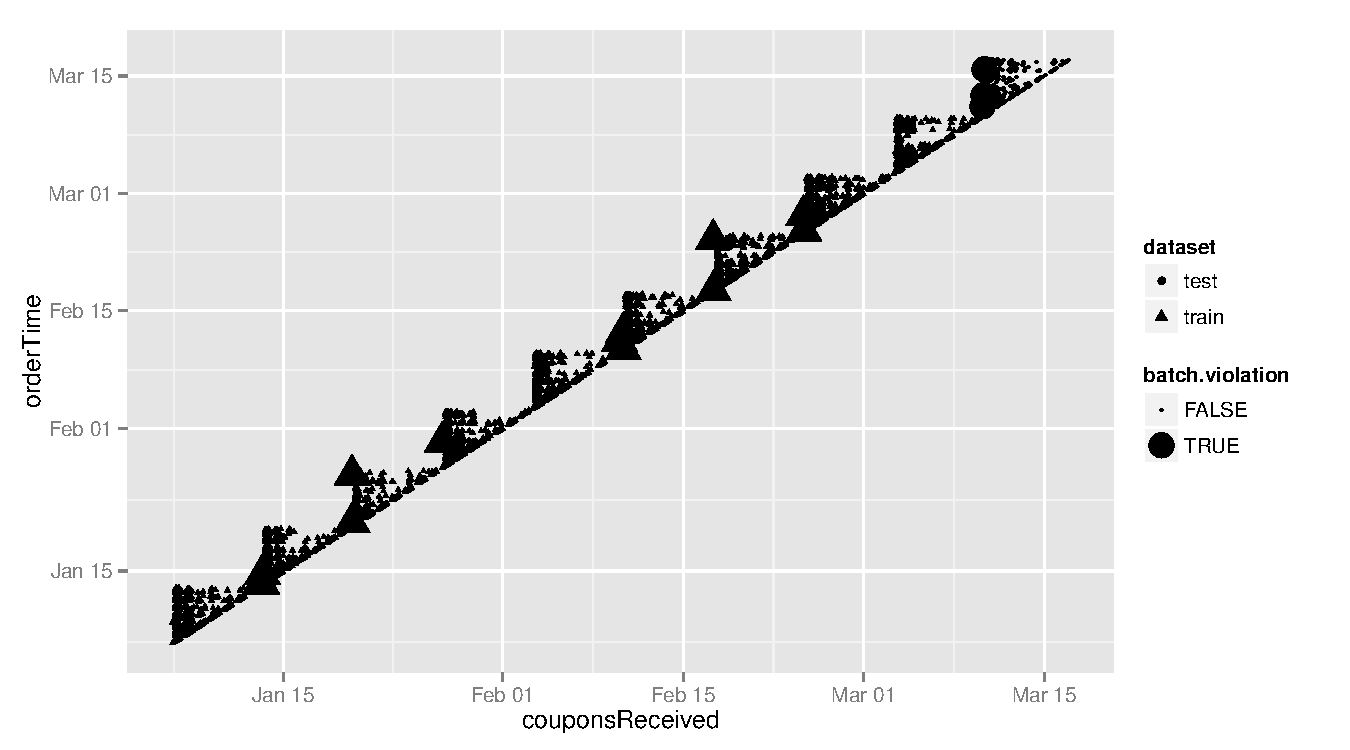
\includegraphics[width=.8\maxwidth]{/Users/user/dmc2015/ian/graphics/graphics_batchplots-1} 
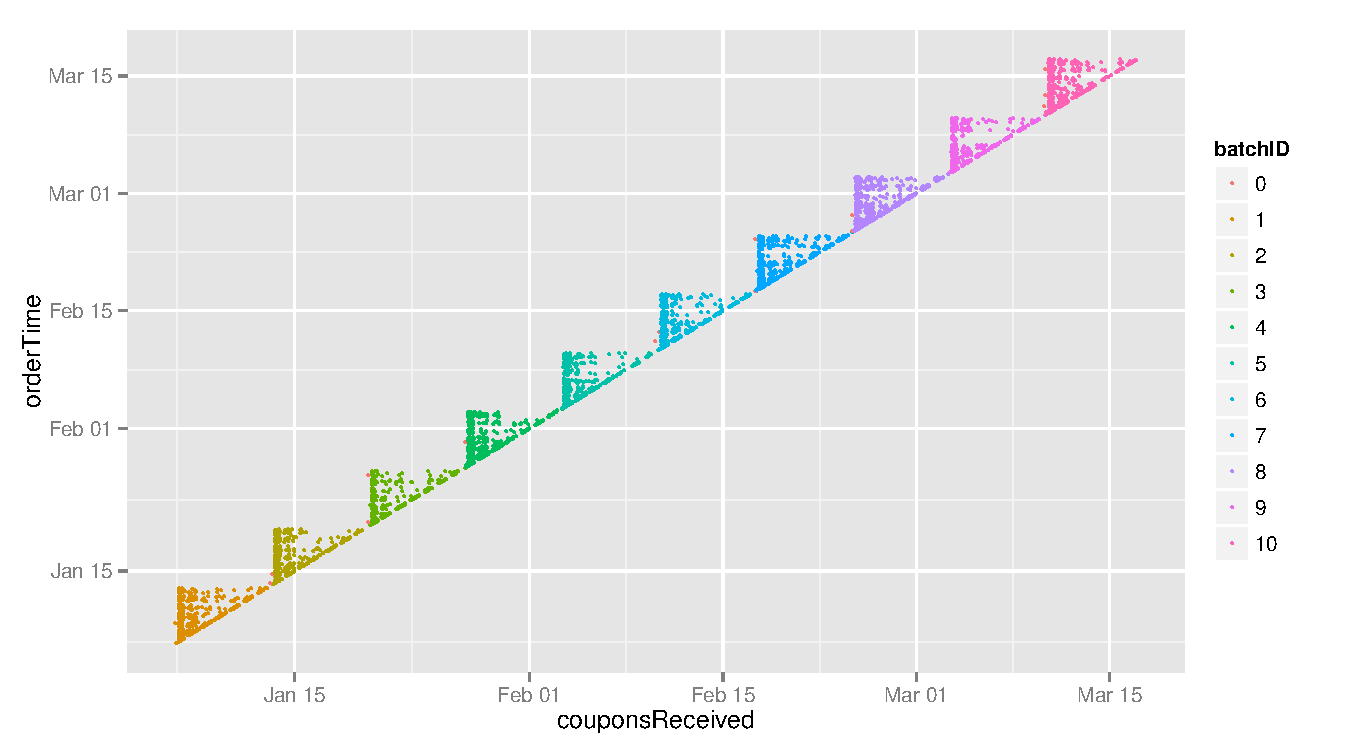
\includegraphics[width=.8\maxwidth]{/Users/user/dmc2015/ian/graphics/graphics_batchplots-2} 
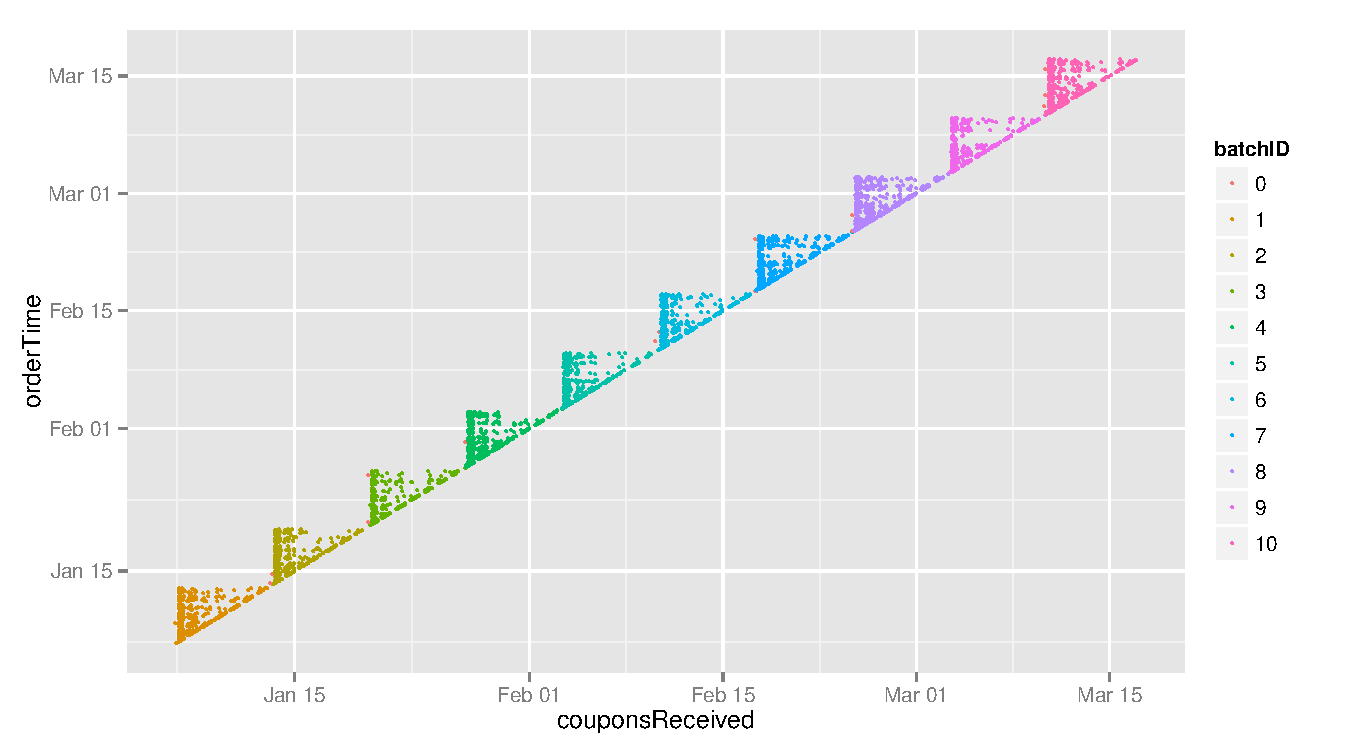
\includegraphics[width=.8\maxwidth]{/Users/user/dmc2015/ian/graphics/graphics_batchplots-3} 

}

\caption[Orders alway follow receiving of coupons, but the odd shapes indicate that there is structure to the data beyond the fact that shoppers get coupons before purchasing any products]{Orders alway follow receiving of coupons, but the odd shapes indicate that there is structure to the data beyond the fact that shoppers get coupons before purchasing any products.}\label{fig:batchplots}
\end{figure}


\end{knitrout}
we may be able to find gaps on the Tuesdays that help us figure out when the coupons are 
and we can plot these as well:
%-- gapsTuesday: R code (Code in Document)
\begin{knitrout}
\definecolor{shadecolor}{rgb}{0.969, 0.969, 0.969}\color{fgcolor}\begin{kframe}
\begin{alltt}
\hlcom{# combine the results}
\hlstd{d} \hlkwb{<-} \hlkwd{rbind}\hlstd{(trn, tst)}

\hlcom{# the only issue is if they get coupons at the very}
\hlcom{# last moment and then order something this means}
\hlcom{# they order coupons on a Tuesday and get coupons}
\hlcom{# on a Tuesday batch.timing =}
\hlcom{# d[which(d$orderTimeDoW == 'Tuesday' &}
\hlcom{# d$couponsReceivedDoW %in%}
\hlcom{# c('Monday','Tuesday')),]}
\hlkwd{min}\hlstd{(d}\hlopt{$}\hlstd{couponsReceivedDate)}
\end{alltt}
\begin{verbatim}
## [1] "2015-01-06 UTC"
\end{verbatim}
\begin{alltt}
\hlkwd{wday}\hlstd{(}\hlkwd{min}\hlstd{(d}\hlopt{$}\hlstd{couponsReceivedDate),} \hlkwc{label} \hlstd{=} \hlnum{TRUE}\hlstd{)}
\end{alltt}
\begin{verbatim}
## [1] Tues
## 7 Levels: Sun < Mon < Tues < Wed < ... < Sat
\end{verbatim}
\begin{alltt}
\hlcom{# start all the weeks between on Sunday}
\hlstd{start.weeks} \hlkwb{<-} \hlkwd{ymd_hms}\hlstd{(}\hlstr{"2015-01-04 00:00:00"}\hlstd{,} \hlkwc{tz} \hlstd{=} \hlstr{"CET"}\hlstd{)}
\hlstd{d}\hlopt{$}\hlstd{StartOfWeek} \hlkwb{<-} \hlstd{start.weeks}
\hlkwa{for} \hlstd{(i} \hlkwa{in} \hlnum{1}\hlopt{:}\hlnum{12}\hlstd{) \{}
    \hlstd{chng} \hlkwb{<-} \hlstd{d}\hlopt{$}\hlstd{couponsReceived} \hlopt{>} \hlstd{start.weeks} \hlopt{+} \hlkwd{weeks}\hlstd{(i)}
    \hlkwa{if} \hlstd{(}\hlkwd{sum}\hlstd{(chng)} \hlopt{>} \hlnum{0}\hlstd{) \{}
        \hlstd{d}\hlopt{$}\hlstd{StartOfWeek[}\hlkwd{which}\hlstd{(chng)]} \hlkwb{<-} \hlstd{start.weeks} \hlopt{+}
            \hlkwd{weeks}\hlstd{(i)}
    \hlstd{\}}
\hlstd{\}}

\hlcom{# lets look for gaps}
\hlstd{b.m} \hlkwb{<-} \hlkwd{melt}\hlstd{(d,} \hlkwd{c}\hlstd{(}\hlstr{"orderID"}\hlstd{,} \hlstr{"couponsReceivedDate"}\hlstd{,}
    \hlstr{"StartOfWeek"}\hlstd{),} \hlkwd{c}\hlstd{(}\hlstr{"orderTime"}\hlstd{,} \hlstr{"couponsReceived"}\hlstd{))}
\hlstd{b.m}\hlopt{$}\hlstd{value} \hlkwb{<-} \hlkwd{as.numeric}\hlstd{(}\hlkwd{difftime}\hlstd{(b.m}\hlopt{$}\hlstd{value, b.m}\hlopt{$}\hlstd{StartOfWeek,}
    \hlkwc{units} \hlstd{=} \hlstr{"days"}\hlstd{))}

\hlstd{DeliveryDates} \hlkwb{<-} \hlkwd{data.frame}\hlstd{(}\hlkwc{daystr} \hlstd{=} \hlkwd{rep}\hlstd{(}\hlnum{0}\hlopt{:}\hlkwd{floor}\hlstd{(}\hlkwd{max}\hlstd{(b.m}\hlopt{$}\hlstd{value))),}
    \hlkwc{dayend} \hlstd{=} \hlkwd{rep}\hlstd{(}\hlnum{1}\hlopt{:}\hlkwd{ceiling}\hlstd{(}\hlkwd{max}\hlstd{(b.m}\hlopt{$}\hlstd{value))),} \hlkwc{lowery} \hlstd{= start.weeks,}
    \hlkwc{uppery} \hlstd{= start.weeks} \hlopt{+} \hlnum{12} \hlopt{*} \hlkwd{weeks}\hlstd{(}\hlnum{1}\hlstd{),} \hlkwc{dow} \hlstd{=} \hlkwd{wday}\hlstd{(start.weeks} \hlopt{+}
        \hlkwd{days}\hlstd{(}\hlnum{1}\hlstd{)} \hlopt{*} \hlstd{(}\hlnum{0}\hlopt{:}\hlkwd{floor}\hlstd{(}\hlkwd{max}\hlstd{(b.m}\hlopt{$}\hlstd{value))),} \hlkwc{label} \hlstd{=} \hlnum{TRUE}\hlstd{,}
        \hlkwc{abbr} \hlstd{=} \hlnum{FALSE}\hlstd{))}

\hlkwd{ggplot}\hlstd{()} \hlopt{+} \hlkwd{geom_rect}\hlstd{(}\hlkwc{data} \hlstd{= DeliveryDates,} \hlkwd{aes}\hlstd{(}\hlkwc{xmin} \hlstd{= daystr,}
    \hlkwc{xmax} \hlstd{= dayend,} \hlkwc{ymin} \hlstd{= lowery,} \hlkwc{ymax} \hlstd{= uppery,} \hlkwc{fill} \hlstd{= dow),}
    \hlkwc{alpha} \hlstd{=} \hlkwd{I}\hlstd{(}\hlnum{0.4}\hlstd{))} \hlopt{+} \hlkwd{geom_line}\hlstd{(}\hlkwc{data} \hlstd{= b.m,} \hlkwd{aes}\hlstd{(}\hlkwc{x} \hlstd{= value,}
    \hlkwc{y} \hlstd{= couponsReceivedDate,} \hlkwc{group} \hlstd{= orderID))}
\end{alltt}
\end{kframe}

{\centering 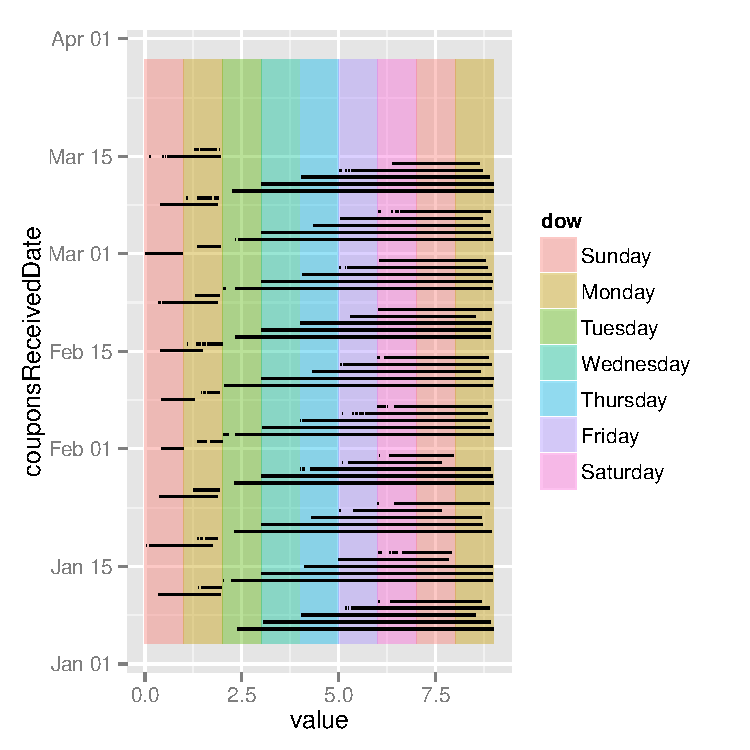
\includegraphics[width=.9\linewidth]{/Users/user/dmc2015/ian/graphics/graphics_gapsTuesday-1} 

}



\end{knitrout}
So using Tuesdays at midnight to demarcate batches seems like a safe solution.
We can save the \verb!order -> batch! assgnments as:
\begin{knitrout}
\definecolor{shadecolor}{rgb}{0.969, 0.969, 0.969}\color{fgcolor}\begin{kframe}
\begin{alltt}
\hlcom{# this batch leads to bad results}
\hlstd{batchres} \hlkwb{<-} \hlkwd{GetBatchInfo}\hlstd{(}\hlstr{"2015-01-06 00:00:00"}\hlstd{)}
\hlkwd{write.csv}\hlstd{(batchres}\hlopt{$}\hlstd{train[,} \hlkwd{c}\hlstd{(}\hlstr{"orderID"}\hlstd{,} \hlstr{"batchID"}\hlstd{,}
    \hlstr{"couponsSent"}\hlstd{,} \hlstr{"couponsExpire"}\hlstd{)],} \hlkwc{file} \hlstd{=} \hlstr{"trainingset.batchID.csv"}\hlstd{,}
    \hlkwc{row.names} \hlstd{=} \hlnum{FALSE}\hlstd{,} \hlkwc{quote} \hlstd{=} \hlnum{FALSE}\hlstd{,} \hlkwc{na} \hlstd{=} \hlstr{""}\hlstd{)}
\hlkwd{write.csv}\hlstd{(batchres}\hlopt{$}\hlstd{test[,} \hlkwd{c}\hlstd{(}\hlstr{"orderID"}\hlstd{,} \hlstr{"batchID"}\hlstd{,} \hlstr{"couponsSent"}\hlstd{,}
    \hlstr{"couponsExpire"}\hlstd{)],} \hlkwc{file} \hlstd{=} \hlstr{"testingset.batchID.csv"}\hlstd{,}
    \hlkwc{row.names} \hlstd{=} \hlnum{FALSE}\hlstd{,} \hlkwc{quote} \hlstd{=} \hlnum{FALSE}\hlstd{,} \hlkwc{na} \hlstd{=} \hlstr{""}\hlstd{)}
\end{alltt}
\end{kframe}
\end{knitrout}
\end{document}
